

\begin{lead}
 本章では,ディジタル信号処理の説明を行うにあたって基礎中の基礎ともいえる
\begin{enumerate}
\item アナログ信号とディジタル信号とのちがい
\item 信号の表現方法
\end{enumerate}
の観点から説明する.

%\end{nerai}

\vfill

%\begin{koumoku}
%アナログフィルタ\\
%ディジタルフィルタ\\
%IIRフィルタ\\
%FIRフィルタ\\
%\end{koumoku}

\end{lead}


\chapter{ディジタル信号}

\label{chapter:3}


%\begin{nerai}

%\clearpage

\section{アナログ信号とディジタル信号}

自然界には種々の信号が存在し,われわれに重要な情報を常に与えている.たとえば,会話においては音声情報が,そして眼に見えてくる情報としては画像情報が不可欠のものである.また,脳波や心電図は身体の健康状態を知るための位置情報であるし,地震波は地震の震源地や規模に関する情報である.このような自然界における信号は,本来,すべてアナログ信号 (analog singal) である.

ところが,近年,このような信号はコンピュータなどに代表されるようなディジタル回路で処理されることが多い\footnote{digitalという言葉をかな表記する場合,電気・電子・情報の分野において,また日本工業規格(JIS)であれば,ディジタルと記すことが一般的である.}
.これは,アナログ回路による処理と比較して,ディジタル回路による処理すなわちディジタル信号処理(digital signal processing)には,多くの利点があるとされているためである.

ディジタル信号処理とは,本来アナログ信号であったものを,ディジタル信号に変換し,コンピュータやディジタル回路を用いて代数的演算(加減算,乗除算)によって処理する方式であり,図\ref{fig:zu-1-1}にその流れを示す.
%
コンピュータはアナログ信号を取り扱うことができないので,アナログ信号をディジタル信号に変換し\footnote{アナログ信号をディジタル信号に変換することを,A-D変換\index{ADへんかん@A-D変換}という.AはAnalog,DはDigitalを意味する.},処理を行うのである.

\begin{figure}[H]
\begin{center}
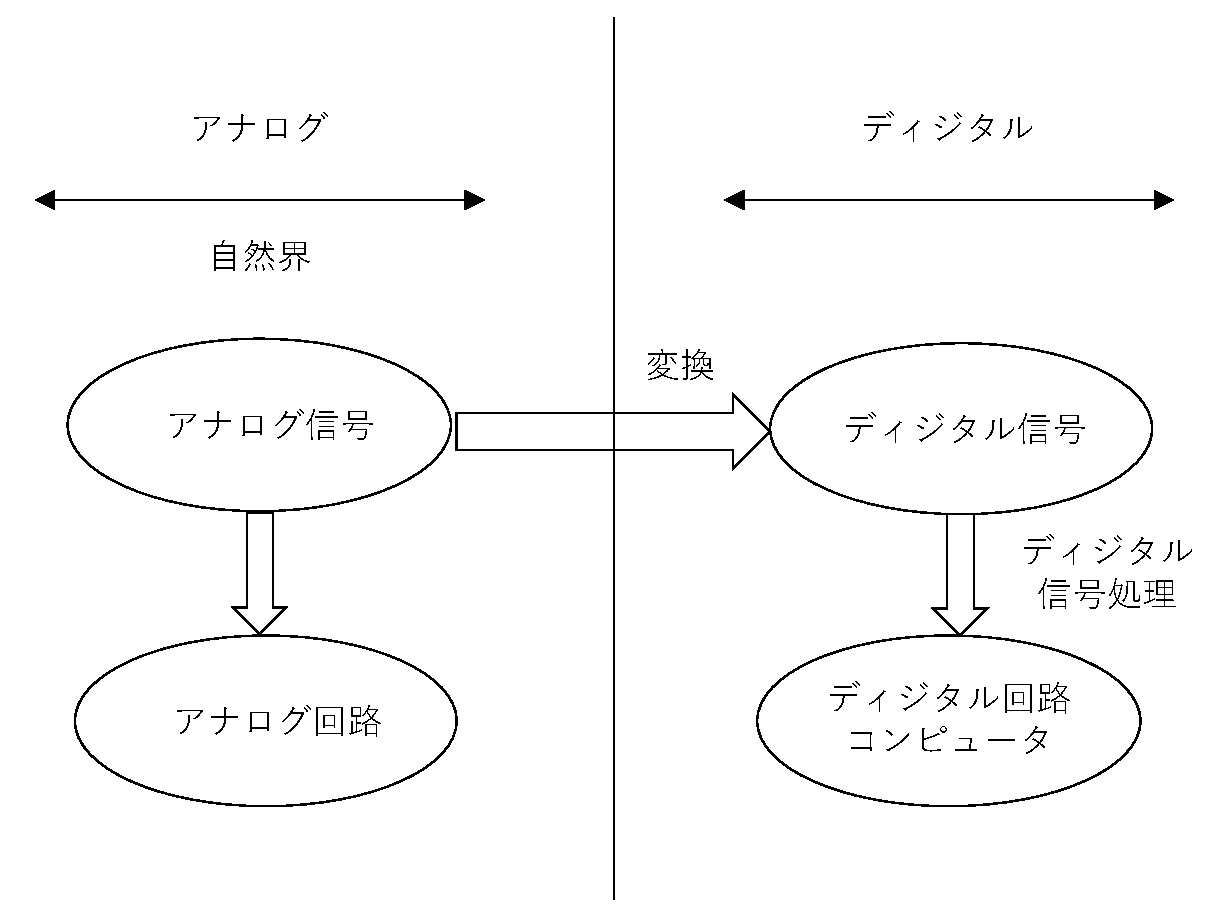
\includegraphics[width=.7\textwidth]{fig/zu-1-1.eps}
\end{center}
\caption{ディジタル信号処理の流れ}
\label{fig:zu-1-1}
\end{figure}


\subsection{信号のサンプリングと量子化}

\subsubsection{正弦波信号}

例として,図\ref{fig:zu-1-2}(a)の信号$x(t)$を考える.この信号は,
\begin{equation}
x(t)=A \sin (\Omega t + \theta)
\label{eqn:eqn-1-1}
\end{equation}
と表現され,正弦波信号と呼ばれる.ただし,$t$は時間(単位は秒:second,secと記される)であり,$\Omega$は角周波数であり,
\begin{equation}
\Omega = 2\pi F \hspace{3mm} \mathrm{[rad / sec]}
\end{equation}
\begin{equation}
F=1/T \hspace{3mm} \mathrm{[Hz]}
\end{equation}
の関係にある.ここで,$T$は正弦波の周期(単位は秒),$F=1/T$は周波数(単位はHz(ヘルツ))である.角度の単位はラジアン(radian,radと記される)であり,360度であれば$2\pi$[rad]である.また,$A$は大きさ(あるいは振幅)であり,$\theta$は初期位相(単位はラジアン)である.

図\ref{fig:zu-1-2}(a)の信号は,式(\ref{eqn:eqn-1-1})において,$A=2$,$F=1$Hz,$\theta=0$radと選んだ場合に相当するので,
\begin{equation}
x(t)=2 \sin (2\pi t)
\label{eqn:eqn-1-2}
\end{equation}
と表現することができる.信号はすべての時間で定義され,大きさが$2$から$-2$の範囲で周期的に変化している様子が確認される.

\begin{figure}[H]
\begin{center}
\begin{minipage}{.38\textwidth}
\begin{center}
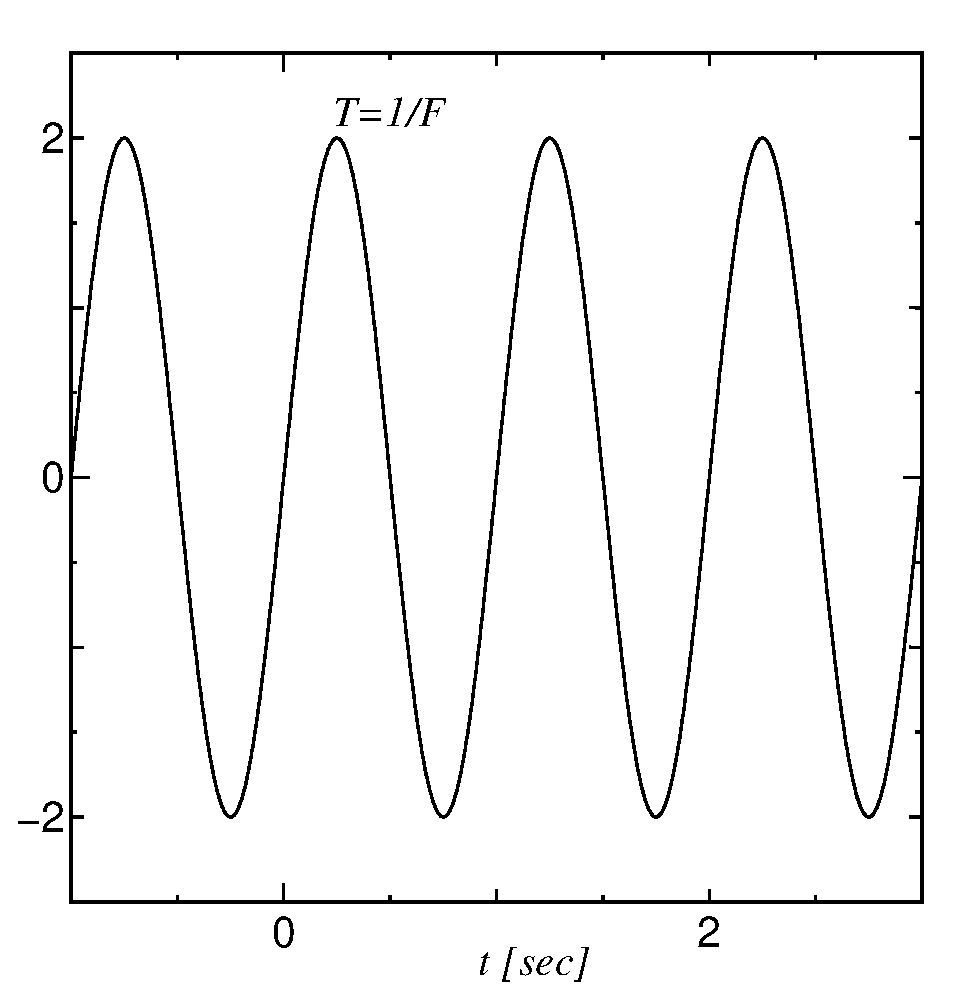
\includegraphics[width=.95\textwidth]{fig/zu-1-2-a.eps}

(a) $x(t)=2 \sin (2\pi t)$
\end{center}
\end{minipage}
\begin{minipage}{.38\textwidth}
\begin{center}
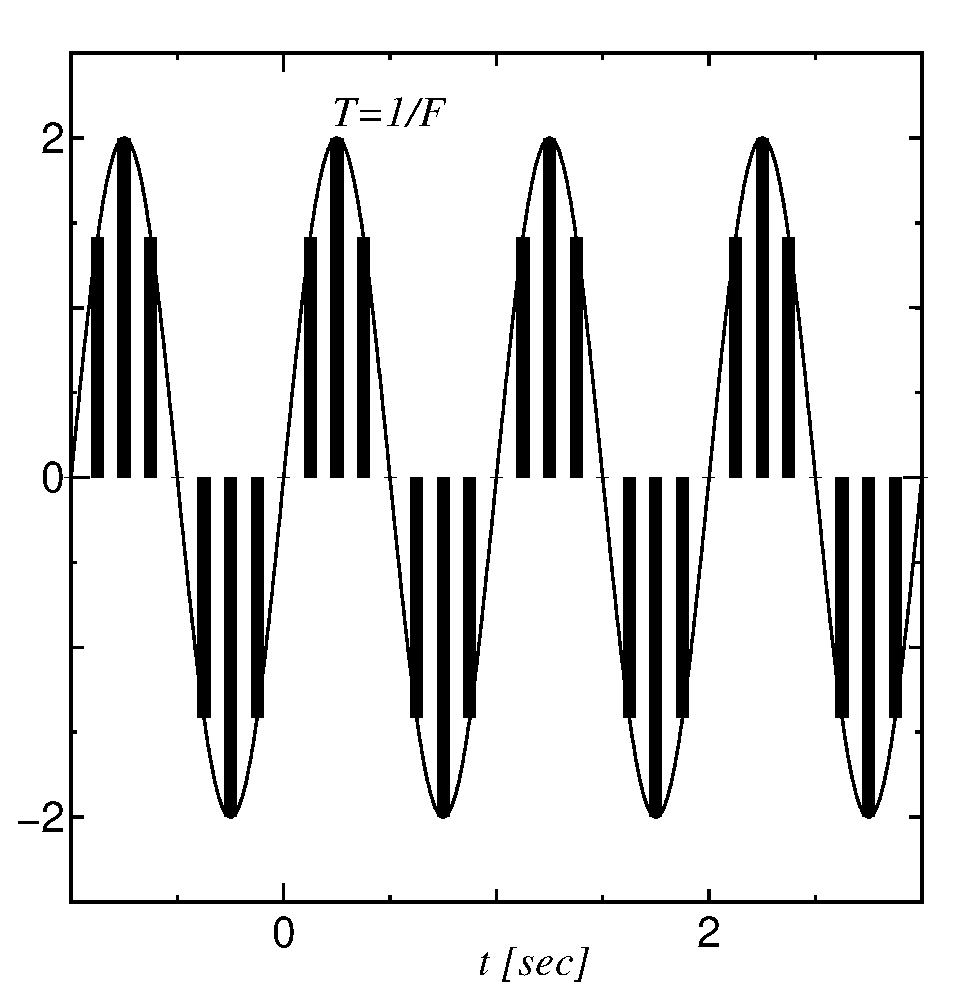
\includegraphics[width=.95\textwidth]{fig/zu-1-2-b.eps}

(b) サンプリング($T=1/8$[sec])
\end{center}
\end{minipage}\\[.5\baselineskip]
\begin{minipage}{.38\textwidth}
\begin{center}
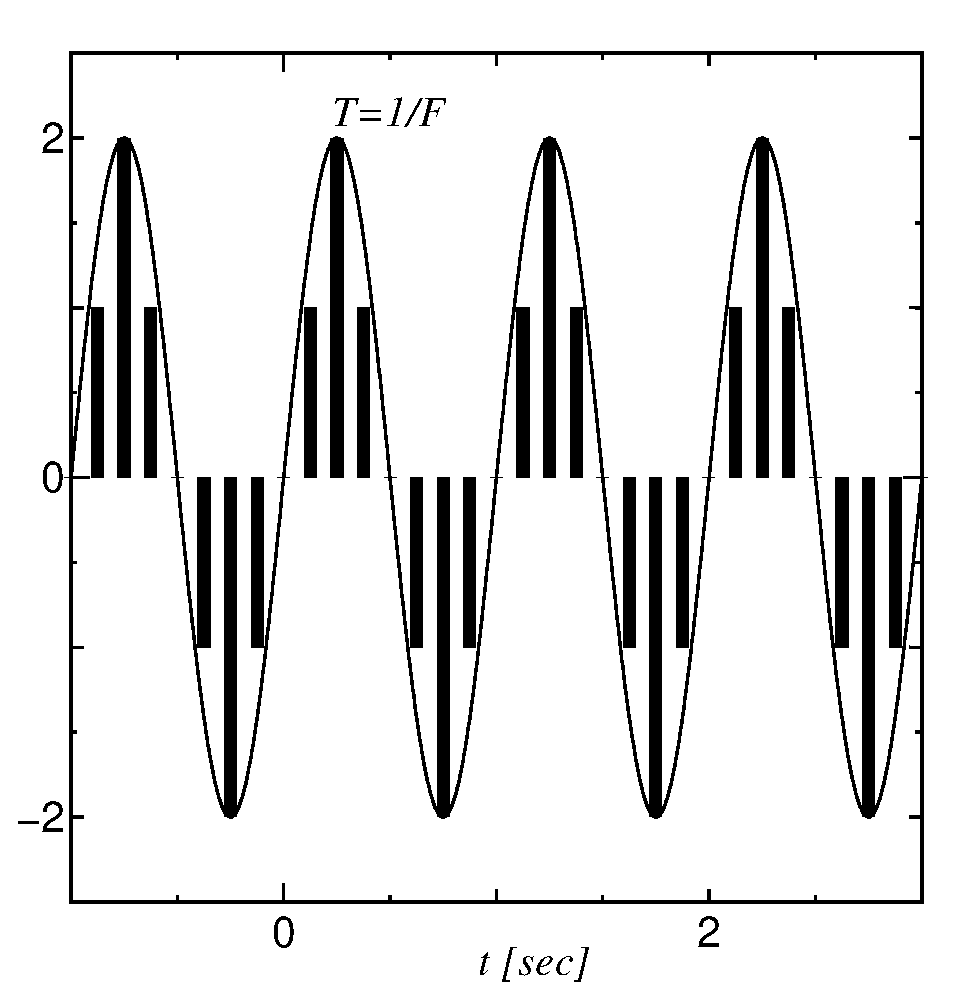
\includegraphics[width=.95\textwidth]{fig/zu-1-2-c.eps}

(c) 量子化
\end{center}
\end{minipage}
\end{center}\vskip.5\baselineskip
\caption{正弦波信号$x(t)=2 \sin (2\pi t)$とサンプリングならびに量子化}
\label{fig:zu-1-2}
\end{figure}

\subsubsection{サンプリング}

正弦波信号$x(t)$から離散的な時間を抽出する操作,すなわち,図\ref{fig:zu-1-2}(a)の波形から図\ref{fig:zu-1-2}(b)を信号を得る操作のことを\index{さんぷりんぐ@サンプリング}サンプリング(sampling,標本化)と呼ぶ.アナログ信号をディジタル信号に変換する際に,最初の段階で必要な操作である.

このサンプリングの操作は,一定の時間間隔$T_s$(これをサンプリング周期(sampling period)またはサンプリング間隔と呼ぶ)で実行される.また,$T_s$の逆数である
\begin{equation}
F_s=1/T_s
\end{equation}
\begin{equation}
\Omega_s=2\pi F_s
\end{equation}
について,$F_s$を\index{さんぷりんぐしゅうはすう@サンプリング周波数}サンプリング周波数(sampling frequency),$\Omega_s$を\index{さんぷりんぐかくしゅうはすう@サンプリング角周波数}サンプリング角周波数(sampling angular frequency)と呼ぶ.サンプリングを行う際に,サンプリング周波数$F_s$をどのような値に選ぶのか,言い換えれば,どのような細かさで信号をサンプリングするかは,実際問題として,非常に重要な課題である.

\subsubsection{量子化}

アナログ信号をディジタル信号に変換する際に,サンプリング操作の次に必要な処理は,\index{りょうしか@量子化}量子化(quantization)である.これは,各サンプル値をたとえば4bitや8bitなどのように,有限な桁数の2進数で表すための操作である\footnotemark .

ところで,図\ref{fig:zu-1-2}(a)の信号を見ると,$x(t)$の大きさの上限は2であり,$x(t)$の大きさの下限は$-2$と決まっている.つまり,$-2 \leq x(t) \leq 2$である.しかしながら,各時刻での入力信号$x(t)$の値は実数をとるために,無限個の種類の値が存在することから,これを2進数で表現することは困難である.

\footnotetext{1ビットの2進数であれば0と1との組合せで2通りである.ところで,2ビットの2進数であれば$2^2=4$通りの組合せまでしか表すことができないが,3ビットの2進数であれば$2^3=8$通りの組合せまでを表すことができる.}

図\ref{fig:zu-1-2}(b)の各サンプル値を5種類の値 ($-2$, $-1$, 0, 1, 2) を用いて実現する場合,5種類の値の組み合わせでもあることから3ビットの2進数で表すことができる.しかし,このサンプル値は,この5種類の値に等しいとは限らないので,各サンプル値に近い値を5種類の値から選び出して,その値によってサンプル値を置き換えるのである.この操作を量子化と呼ぶが,具体的な方法のひとつは,図\ref{fig:zu-1-2}(c)のように,各サンプル値を小数点第1位で四捨五入して,5種類の値に置き換えることである.それを式として表現すると,
\begin{equation}
s(nT_s)=\mathrm{round} \left [ \frac{x(nT_s)}{\Delta}\right ]
\end{equation}
のようになる.ここで$\mathrm{round[y]}$は,値$y$を小数点以下四捨五入する操作という意味であり,$\Delta$は量子化ステップである.この例の場合であれば,$-2 \sim 2$までの間で1刻みの間隔であることから$\Delta=1$である.また,この量子化を行うときに発生する誤差$x(nT_s) - s(nT_s)$を量子化誤差 (quantization error) と呼ぶ.

\subsection{信号の分類}

信号のサンプリングと量子化について先述したので,いったん,時間と信号の大きさに関する連続性について着目すると,表\ref{table:table-1-2}のように分類される.

\begin{table}[t]
\caption{信号の分類}
\label{table:table-1-2}
\begin{center}
\begin{tabular}{|c|c|c|c|}
\hline
 \multicolumn{1}{|c}{} & \multicolumn{1}{c}{} & \multicolumn{2}{|c|}{大きさ} \\ \cline{3-4}
 \multicolumn{1}{|c}{} & \multicolumn{1}{c|}{} & 連続 & 離散 \\
\hline
 時間 & 連続 & アナログ信号 & 多値信号 \\ \cline{3-4}
 & & \multicolumn{2}{|c|}{連続時間信号} \\ \cline {2-4}
 & 離散 & サンプル値信号 & ディジタル信号 \\ \cline {3-4}
 &  & \multicolumn{2}{|c|}{離散時間信号} \\ \hline
\end{tabular}
\end{center}
\end{table}

ここで,大きさが離散的であるとは,大きさを有限桁の2進数で表現できるという意味である.時間に関して連続的であれば\index{れんぞくじかんしんごう@連続時間信号}連続時間信号 (continuance-time signal) と呼び,\index{あなろぐしんごう@アナログ信号}アナログ信号と\index{たちしんごう@多値信号}多値信号とを総称している.一方,時間に対して離散的であれば離散時間信号 (discrete-time signal) と呼び,サンプル値信号とディジタル信号とを総称している.

信号処理の内容を講述するにあたっては,多くの場合,サンプル値信号とディジタル信号とを区別せず,離散時間信号という表現を用いることが多く,本書でもこの表現をしばしば用いている.

\section{信号の表現法}

ここでは離散時間信号の数式表現について説明する.

\subsection{離散時間信号の表現}

引き続き,図\ref{fig:zu-1-2}(a)の正弦波信号を例にして,離散時間信号の数式表現を導く.図\ref{fig:zu-1-2}(a)の正弦波信号は,
\begin{equation}
x(t)=A \sin (\Omega t)
\label{eqn:eqn-1-7}
\end{equation}
と表現される.いま,サンプリング周期$T_s$でこの信号をサンプリングするとき,図\ref{fig:zu-1-5}(a)の信号が生成される.この離散信号の表現は,式(\ref{eqn:eqn-1-7})の時間$t$に離散時間$nT_s$($n$:整数)を代入することにより,
\begin{equation}
x(nT_s)=A \sin (\Omega nT_s)
\label{eqn:eqn-1-8}
\end{equation}
と表現される.ここで,$n$の値を0,1,2,$\cdots$と選ぶことにより,各サンプル値が対応する.

\subsection{信号の正規化表現}

ここで,式(\ref{eqn:eqn-1-8})の\index{りさんじかんしんごう@離散時間信号}離散時間信号を,より簡潔に表現するために,
\begin{equation}
x(n)=A \sin (\omega n)
\label{eqn:eqn-1-9}
\end{equation}
と表す.この表現を離散時間信号の正規化表現という.ここで,式(\ref{eqn:eqn-1-8})と式(\ref{eqn:eqn-1-9})には,2つの相違点が見られることがわかる.

第1の相違点は,\index{さんぷりんぐしゅうき@サンプリング周期}サンプリング周期$T_s$が式(\ref{eqn:eqn-1-9})のなかで省略されていることである.これは,図\ref{fig:zu-1-5}(b)に示すように時間$t$を整数$n$で置き換え,各サンプル値に番号を付した時系列としての表現を意味する.

第2の相違点は,\index{かくしゅうはすう@角周波数}角周波数$\omega$の扱いである.これは,角周波数$\Omega=2\pi F$と,
\begin{equation}
\omega=\Omega T_s=\Omega / F_s \mathrm{[rad]}
\label{eqn:eqn-1-10}
\end{equation}
\begin{equation}
f=\frac{\omega}{2\pi}=\frac{F}{F_s}
\label{eqn:eqn-1-11}
\end{equation}
の関係にある.つまり,非正規化表現$(\Omega,F)$を\index{さんぷりんぐしゅうはすう@サンプリング周波数}サンプリング周波数$F_s$で割った表現であると解釈することができる.ここで,$\omega$を正規角周波数(normalized angular frequency)と呼ぶ.これはサンプリング周期あたりの角度に相当するもので,単位は[rad]である.また,$f$を正規化周波数とよび,式(\ref{eqn:eqn-1-11})に示されるように,通常は無次元である.

本書においては,正規化表現を$(f,\omega)$,非正規化表現を$(\Omega, F)$により表現するものとして,議論を進めるものとする.

\begin{figure}[H]
\begin{center}
\begin{minipage}{.4\textwidth}
\begin{center}
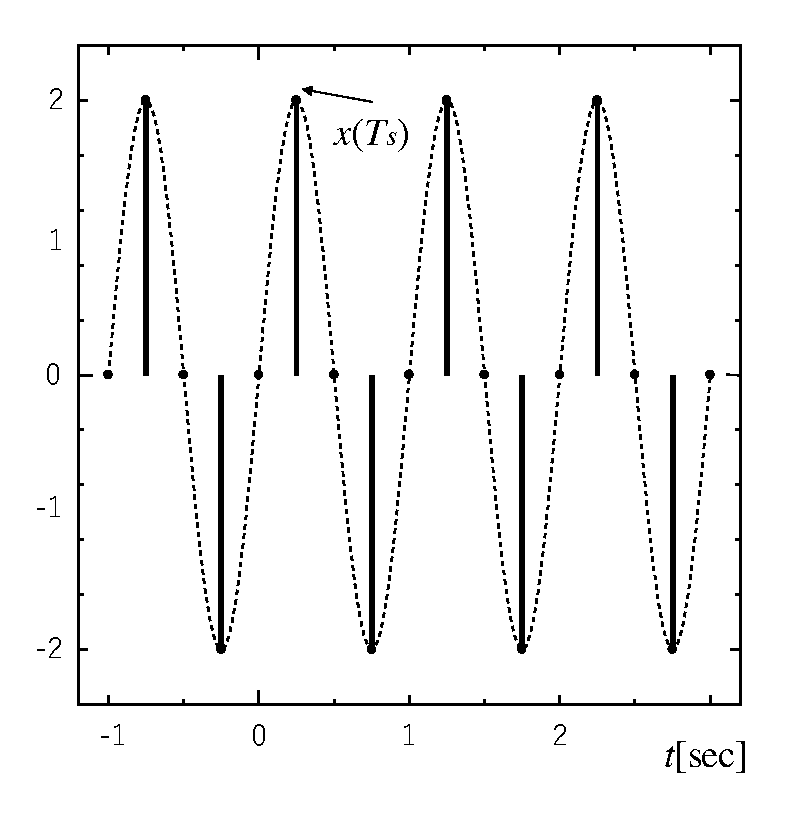
\includegraphics[width=.95\textwidth]{fig/zu-1-5-a.eps}

(a) 非正規化表現:\\ $x(nT_s)=A \sin (\Omega n T_s)$
\end{center}
\end{minipage}
\begin{minipage}{.4\textwidth}
\begin{center}
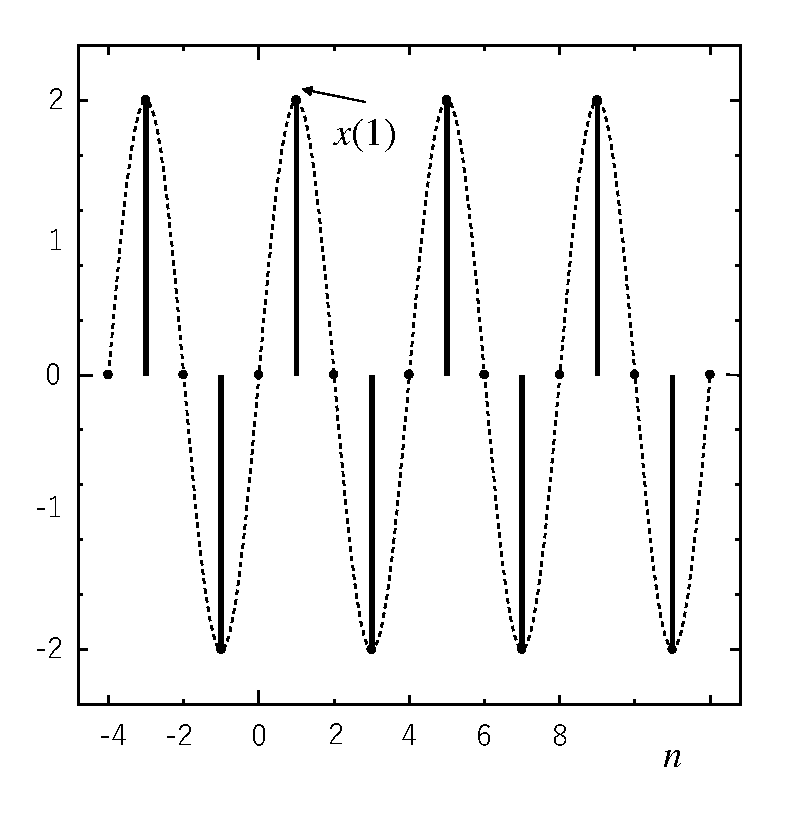
\includegraphics[width=.95\textwidth]{fig/zu-1-5-b.eps}

(b) 正規化表現:\\ $x(n)=A\sin (\omega n)$
\end{center}
\end{minipage}
\end{center}\vskip.5\baselineskip
\caption{信号の正規化表現$(A=2, \Omega=2\pi F, F=1, T_S=1/4)$}
\label{fig:zu-1-5}
\end{figure}

\section{信号の処理手順}

ここでは,信号をディジタル信号として処理するための手順を示し,アナログ信号処理と比較したディジタル信号処理の利点を示す.

\subsection{ディジタル信号処理の処理手順}

図\ref{fig:zu-1-7}は,ディジタル信号処理における標準的な処理手順を示したものである.この処理手順の概略は以下の通りである.
\begin{enumerate}
\item アナログフィルタ(低域フィルタ)によって,アナログ信号の高周波成分を除去する.
\item 帯域制限されたアナログ信号を,A-D(アナログ$-$ディジタル)変換器によりディジタル信号に変換する.
\item ディジタルシステムによって,目的である信号処理を行う.
\item D-A(ディジタル$-$アナログ)変換器によって,アナログ信号に戻す.
\item \index{あなろぐふぃるた@アナログフィルタ}アナログフィルタ(\index{ていいきふぃるた@低域フィルタ}低域フィルタ)を用いて,信号を平滑化する.
\end{enumerate}

上記のような手順によるディジタル信号処理の詳細を学ぶということは,これらの処理順の必要性や,各処理における具体的実行法を学ぶことでもある.これらの詳細は章を改めて説明する.

\begin{figure}[H]
\begin{center}
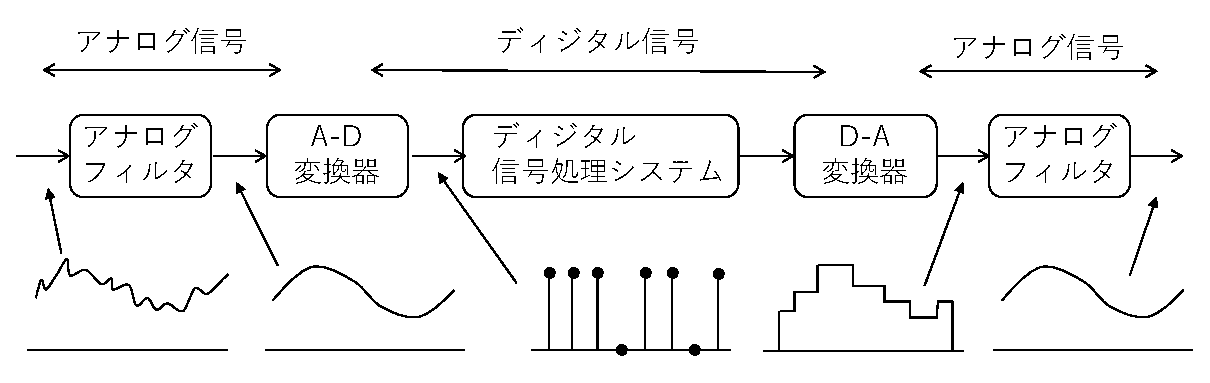
\includegraphics[width=.8\textwidth]{fig/zu-1-7.eps}
\end{center}
\caption{ディジタル信号処理の処理手順}
\label{fig:zu-1-7}
\end{figure}

\subsection{ディジタル信号処理の利点}

ディジタル信号処理は,アナログ信号処理と比較して,主に以下に示すような優れた特徴を持っている.
\begin{enumerate}
\item 経済性と信頼性の向上\\
ディジタル信号処理の技術は,高精度で信頼性の高い製品を経済的に開発することが可能となる.具体的には以下の通りである.
\begin{enumerate}
\item \index{LSIぎじゅつ@LSI技術}LSI技術に基づくことにより,大量生産の際の製品の低価格化が可能
\item LSI技術により,製品の小型化,高信頼化が可能
\item ディジタルという観点から,温度変化や経年変化に対して安定性が向上
\item ソフトウェアの併用により,仕様の変更や開発期間の短縮が可能
\end{enumerate}
\item 信号処理の多様化\\
アナログ信号処理では,以下のような複雑で困難な処理を行うことができる.
\begin{enumerate}
\item コンピュータやディジタルメモリを用いた,複雑で汎用性の高い処理
\item データの圧縮,データのセキュリティ化など
\item 並列処理,非線形処理など
\end{enumerate}
\end{enumerate}

以上の特徴を考えると,ディジタル信号処理の内容を理解すれば,マルチメディア信号などの処理も理解することが可能となるのである.

\section*{演習問題}
%解答は記述済み

\subsection*{問題\ref{chapter:3}.1}

以下の信号を時間$n$を横軸として図に示せ.

(1) $x(n)=-\delta(n+2)+2\delta(n)+\delta(n-1)+\delta(n-1)$

(2) $x(n)=u(n)-u(n-3)$

(3) $x(n)=u(-n)-u(n+3)$


\subsection*{問題\ref{chapter:3}.2}

サンプリング周波数$F_s=44.1$kHzの場合,サンプリング間隔$T_s$はいくらか.

\subsection*{問題\ref{chapter:3}.3}

図\ref{fig:zu-1-7}においてアナログフィルタが用いられている理由を説明せよ.



